\chapter{B Tagging Studies}
\label{c:b_tagging_studies}

Since the \tquark decays to a \W boson and a \bquark, the understanding of these decay products is important
in studies of \ttbar events. In particular, methods to identify jets coming from a \bquark, known as
\btagging, are commonly used to increase the efficiency of a signal selection. CMS has several algorithms for
\btagging: TrackCounting (High Efficiency) and TrackCounting (High Purity), JetBProbability; JetProbability;
SoftMuon; SoftMuonByPt; SoftMuonByIP3d; SimpleSecondaryVertex (High Efficiency); SimpleSecondaryVertex (High
Purity); CombinedSecondaryVertex; CombinedSecondaryVetexMVA. These algorithms produce a discriminator output
for each jet which indicates how likely it is to be a \b flavour jet. In all cases, a more positive
discriminator value indicates a jet that is more likely to be a \b flavour jet. Performance of the different
algorithms varies owing to the fact that they use different jet properties to produce their discriminators.

\section{Inputs to \btagging algorithms}
\label{s:inputs_to_btagging_algorithms}

\subsection{Vertex Finding}
\label{ss:vertex_finding}


\subsection{Impact Parameter}
\label{ss:impact_parameter}


\section{Algorithm descriptions}
The JetProbability algorithm calculates the signed impact parameter significance based on all good tracks in
the jet, and uses this significance to calculate discriminator based on the confidence level that all tracks
are from the primary vertex. The JetBProbability variant of this algorithm uses only the four most displaced
tracks in the jet.

The Simple Secondary Vertex uses an adaptive vertex finder to reconstruct the secondary vertex and
calculate the disciminator based on variables such as the decay length significance.

The Soft Muon algorithms
use the detection of a muon from the semi-leptonic decay of a b quark and a neural net analysis. The Track
Counting algorithms simply take all the tracks within a jet and order them by decreasing order of signed
impact parameter significance, with the discriminator being the significance of the second track (high efficiency) or
the third track (high purity).

The current CMS recommendation is to use the Combined Secondary Vertex (CSV) algorithm for physics analyses.
This algorithm reconstructs the event vertices using the Trimmed Kalman Vertex Finder, which fits tracks to a
primary vertex after removing incompatible tracks and applies cuts to these vertices in order to find a
secondary vertex (the \b decay vertex). Depending on how many candidate secondary vertices are found,
different combinations of variables such as impact parameter, flight distance significance between primary and
secondary vertices, event kinematics and secondary vertex information are used to calculate a discriminator
value \cite{CSV}.

TODO: INCLUDE A MORE DETAILED DESCRIPTION OF EACH ALGORITHM? ALSO INCLUDE PLOTS FOR OTHER ALGORITHMS?
%TODO: INCLUDE A MORE DETAILED DESCRIPTION OF EACH ALGORITHM?

\section{Algorithm analysis}
\label{s:algorithm_analysis}

Analysing a Fall 2011 \ttbar Madgraph Monte Carlo sample (/TTJets\_TuneZ2\_7TeV-madgraph-tauola/) simulated in
CMSSSW 44X, all algorithms produced higher discriminator values for the b jets in the sample than the light
jets (up, down and strange flavour), gluon jets and c flavour jets. All histograms were normalised to unity in
order to facilitate shape comparison. Figure~\ref{fig:CSV_discriminators} shows these normalised histograms
produced by the CSV algorithm.

\begin{figure}[hbtp]
   \centering
     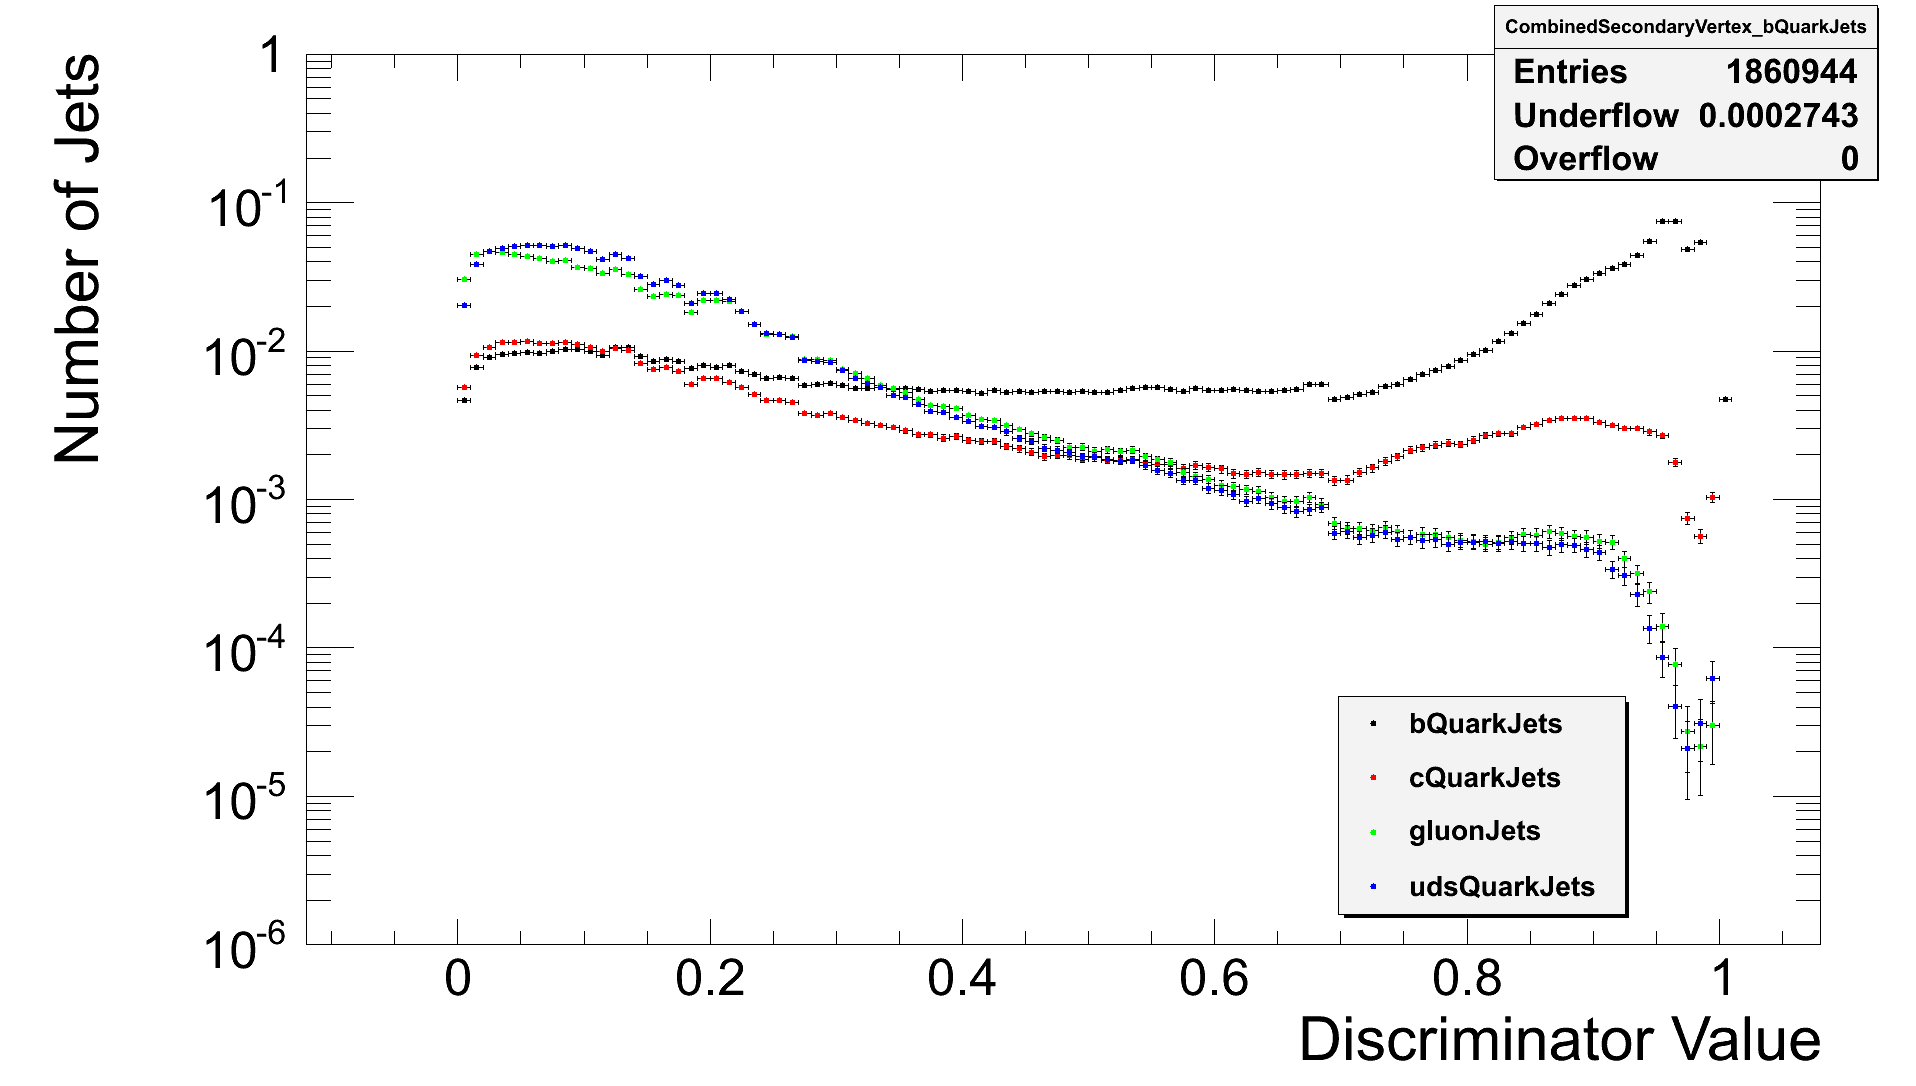
\includegraphics[width=\textwidth]{Chapters/04_Analysis/04a_BTags/Images/CombinedSecondaryVertex_discriminator_combined}\\
     \caption{Discriminator values produced by the Combined Secondary Vertex algorithm for all 4 jet flavours after normalisation}
     \label{fig:CSV_discriminators}
\end{figure}

\section{Efficiency}
\label{s:efficiency}

Cutting on a desired discriminator value allows the efficiency of that cut value to be found by taking the
area of the histogram to the right of the cut value, as a proportion of the total histogram area. Cuts were
made through the whole range of discriminator values in order to create plots of b tag efficiency as a
function of cut value. In practice, the aim is to acheive a high efficiency for b jets and a low efficiency
for all other jet flavours. Figure~\ref{fig:jet_efficiencies} shows how the efficiency for light, gluon and c
jets vary as a function of b jet efficiency for cuts made on the CSV discriminator.

\begin{figure}[hbtp]
   \centering
     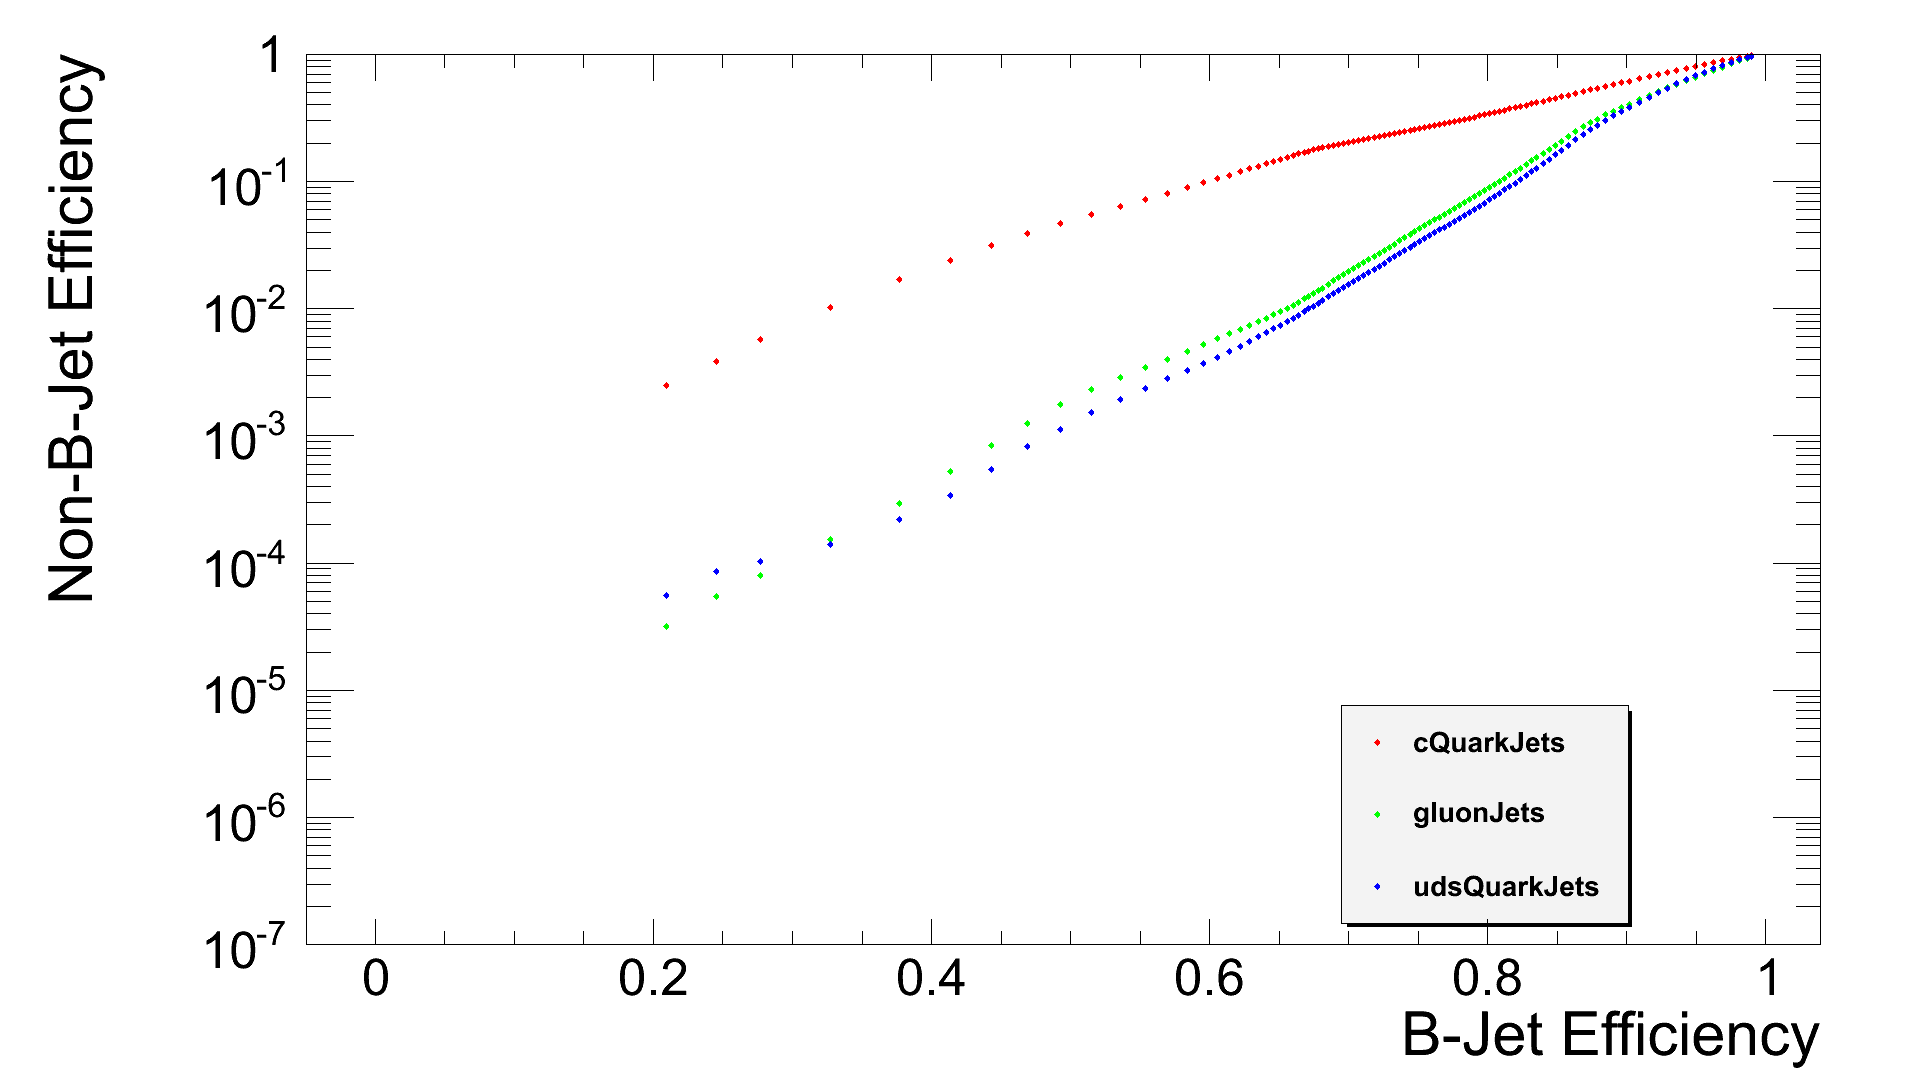
\includegraphics[width=\textwidth]{Chapters/04_Analysis/04a_BTags/Images/CombinedSecondaryVertex_nonBJetEfficiency_v_BJetEfficiency}\\
     \caption{Non b jet effiencies as a function of b jet efficiency for the CSV algorithm}
     \label{fig:jet_efficiencies}
\end{figure}

\section{Algorithm Comparison}
\label{algorithm_comparison}

The performances of the various algorithms can be compared in Figure~\ref{fig:uds_eff_v_b_eff}.

\begin{figure}[hbtp]
   \centering
     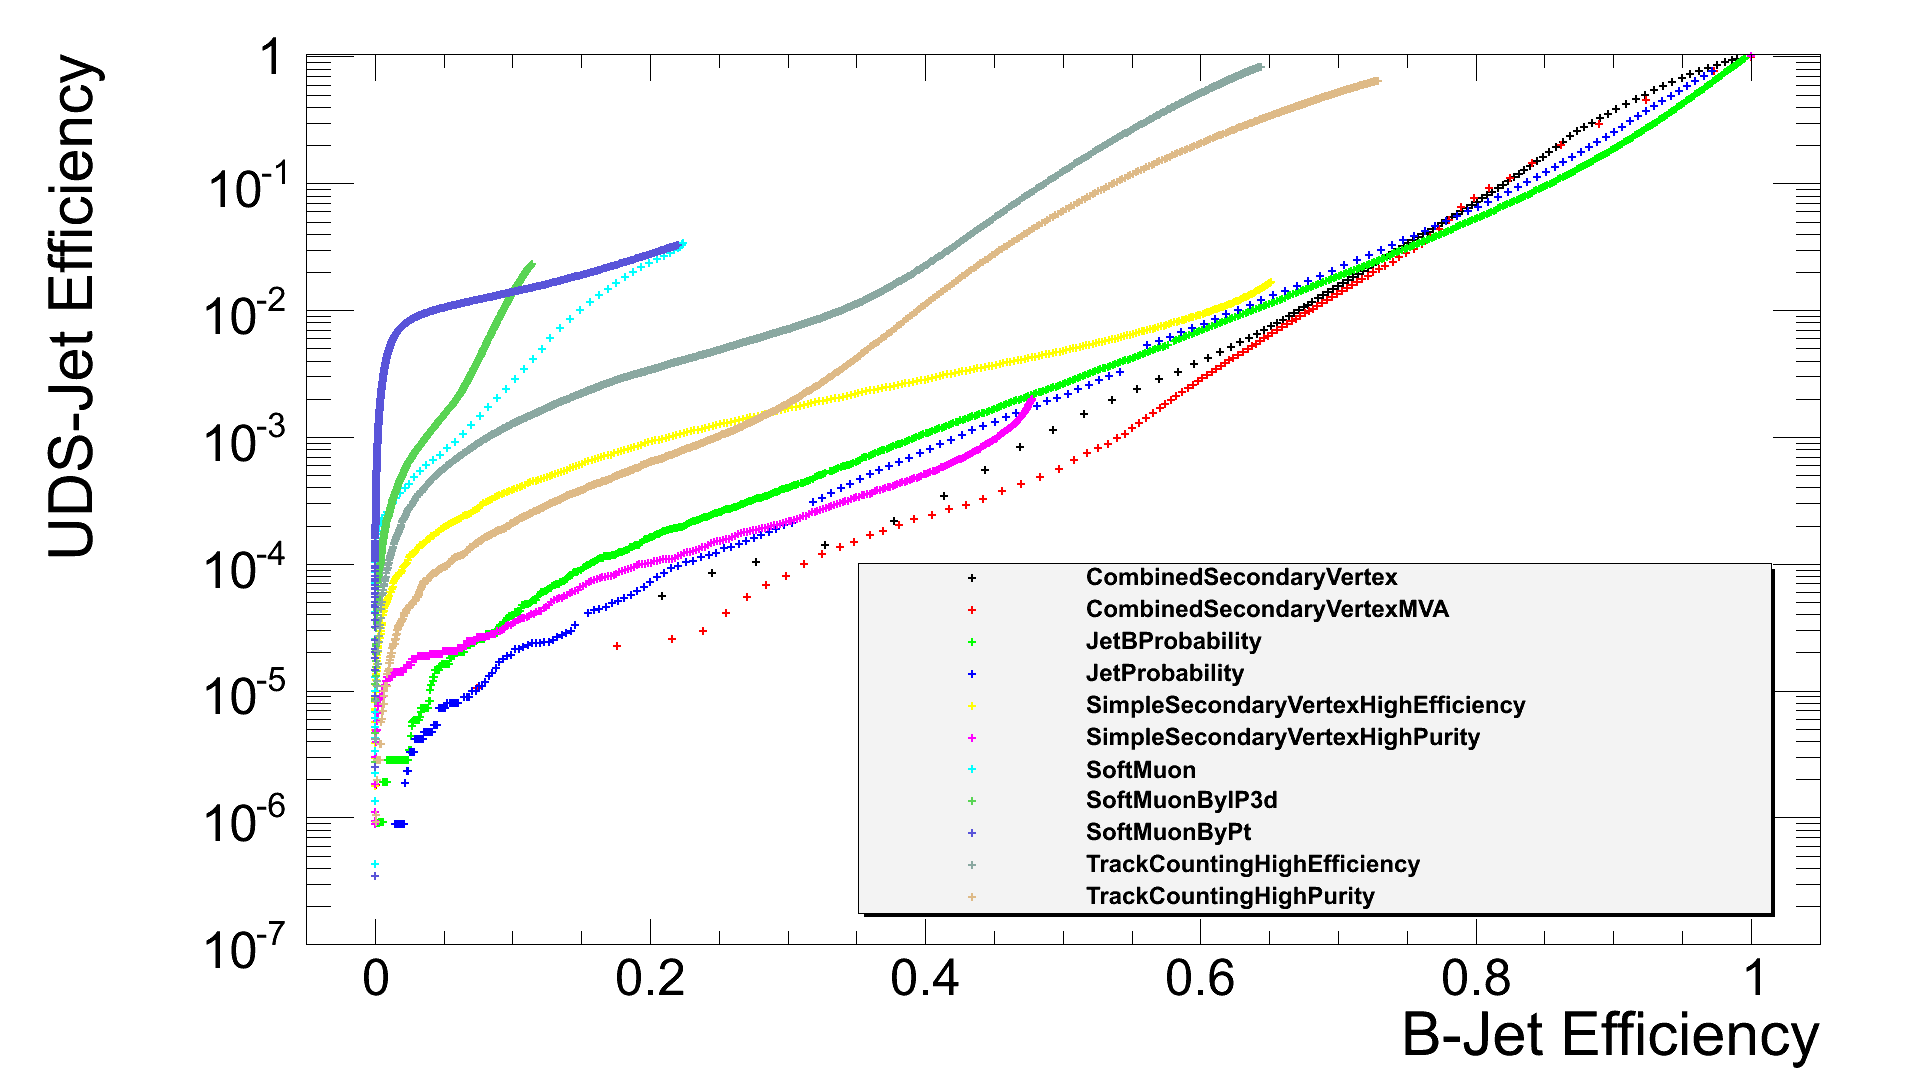
\includegraphics[width=\textwidth]{Chapters/04_Analysis/04a_BTags/Images/UDS-JetEfficiency_v_B-JetEfficiency_withLegend}\\
     \caption{UDS jet efficiencies as a function of b jet efficiencies for all algorithms}
     \label{fig:uds_eff_v_b_eff}
\end{figure}

Algorithms which reach closest to the lower lower right of the plot show better performance, according to the
requirements of high b jet efficiency and low light jet efficiency. It can be seen that not all algorithms
reach 100\% efficiency for b jets due to some being inherently limited by their methods EXPAND ON THIS. For
instance, the soft muon algorithms all show low maximum b jet efficiencies due to the low b hadron semi
leptonic branching ratio to muon of approximately 11\% (or 20\% when further decays are included)
\cite{btagging_in_CMS}. The 2011 and 2012 CMS recommended b tagger is the Combined Secondary Vertex with
operating point cuts of 0.244 (loose), 0.679 (medium) and 0.898 (tight) corresponding to 10\%, 1\% and 0.1\%
light jet and gluon jet efficiencies respectively. These cuts are indicated by the horizontal lines on
Figure~\ref{fig:uds_eff_v_b_eff}. It can be seen that for the tight and medium cuts, the CSV MVA algorithms
provides highest b jet efficiency and lowest light jet efficiency, followed closely by the CSV algorithm. At
approximately 3\% light jet efficiency, there is a convergence of many b taggers which all provide similar
performance, above which the JetBProbability algorithm gives marginally highger b jet efficiency.

